%\documentstyle[nips14submit_09,times,art10]{article} % For LaTeX 2.09
\documentclass{article} % For LaTeX2e
\usepackage{nips14submit_e,times}
\usepackage{hyperref}
\usepackage{url}
\usepackage{subcaption}

\usepackage{amsmath}
\usepackage{framed}
\usepackage{color}
\definecolor{shadecolor}{gray}{0.8}

\usepackage{natbib}
\bibliographystyle{apalike}

\usepackage{tikz}
\usetikzlibrary{bayesnet}

\renewcommand\phi\varphi
\DeclareMathOperator*{\argmax}{arg\,max}

\title{Inducing Semantic Frames on a Very Large Corpus of Syntactic-Ngrams}

\author{
    Noble, Bill\\
    \texttt{winobes@gmail.com}
    \and
    Drumm, Eli T.\\
    \texttt{etd@dte.li}
    \and
    Verdegaal, Jacob\\
    \texttt{jacob.verdegaal@student.uva.nl}
}

% The \author macro works with any number of authors. There are two commands
% used to separate the names and addresses of multiple authors: \And and \AND.
%
% Using \And between authors leaves it to \LaTeX{} to determine where to break
% the lines. Using \AND forces a linebreak at that point. So, if \LaTeX{}
% puts 3 of 4 authors names on the first line, and the last on the second
% line, try using \AND instead of \And before the third author name.

\newcommand{\fix}{\marginpar{FIX}}
\newcommand{\new}{\marginpar{NEW}}

\nipsfinalcopy % Uncomment for camera-ready version

\begin{document}


\maketitle


\begin{abstract}
The abstract paragraph should be indented 1/2~inch (3~picas) on both left and
right-hand margins. Use 10~point type, with a vertical spacing of 11~points.
The word \textbf{Abstract} must be centered, bold, and in point size 12. Two
line spaces precede the abstract. The abstract must be limited to one
paragraph.
\end{abstract}

\section{Introduction}
When a machine looks at the sentence \textit{'Alice buys a bread from the baker'} it does not know it descibes the exact same situation as \textit{`The baker sells Alice a bread'}. But for a lot of applications it is usefull to have semantic representations of senteces or groups of sentences. For example in automatic summarization, some sentences are repaeated with different word choices and orders to express nuances, but since nuances can be left out in summarizations it would be usefull to have techniques to represent and generate semantic content. 

The Framenet project \citep{framenet} is ongoing on defining frames manually which could be mapped on a text to extrct frames. But with the increasing amount of digital information it is usefull to have auomatic semantic frame induction. For example for automatic stock trading systems, it would be usefull to know what is published about companies that are traded on. 

Semantic content of texts can be represented in frames, where the head of the frame represents the core of the episode and roles in the frame espress involement of things or people, location, time etc. For the sentences above the frame would look like this:\\

\begin{table}[h]
\centering
\begin{tabular}{|l l|}
  \hline
  \textit{\small predicate:\normalsize}&Transaction\\
  \hline
  \hline
  \textit{\small role 1:\normalsize} &baker\\
  \textit{\small role 2:\normalsize} &Alice\\
  \textit{\small role 3:\normalsize} &bread\\
  \hline
\end{tabular}
\end{table}

The head of the frame, representing the core of the episode, can naturally be represented as a predicate but the trick is to find out which words have which roles. In linguistics this is called case grammar \citep{dowty1991}. As the example above shows, the roles are represented by different syntactic parts of speech in both sentences, the object and subject are switched, furthermore, the verbs are different. But even with knowledge of specific vebrs which bear the same meaning with switched subject/indirect-object, we need to have technology to let machines generate semantics next to syntacs in order to let machines be able to ( do as if they ) understand language and process new text in a meaningfull way. Hence, automatic semantic analysis and representation is required.\\ 

In this project we investigate wheter probabalistic latent-variable models can cluster verbs (as being a predicate) based on their meaning, which is inferred from the occurences of arguments it is encountered with. The clusters then make up the broader meaning of the predicates. The data we use contains triples of verb-subject-object (see section\ref{data}), so induced frames contain only two roles. The models (described in section \ref{models}) induce frames based on the assumption the meaning of a verb relative to meaning of other verbs can be induced from its context. Hence the broader meaning is latent. To evaluate our models we use two metrics, one of which uses framenet data, the other to check wheter the resulting frames are coherent. See section \ref{results} for more detail.

%\section{Related Work}
We based our work on two papers: \textit{`Inducing a semantically annotated lexicon via em-based clustering.'} by \citeauthor{rooth1999} and \textit{`Learning frames from text with an unsupervised latent variable model.'} by \citeauthor{oconnor2013}. In the first article clustering is realized by applying expectation maximalization on a simple model. This model produces frames in the form of 3 distributions, one for the predicate and two for the arguments. Frame assignement is result of calculating  probabilities for a given tuple, the frame that gives the highest probaility is then the assigned. We will use this model as our baseline (as in the O'Connor paper). The second paper covers multliple models of which we implemented one. The difference with the baseline model is the assumption that a document uses a set of frames repeatedly as a rsult of a document having a (couple of) topics. In our data the tuples are not annotated with documents so we used this assumption in such a way that each verb covers one document.  


\section{Induction Models}
\label{models}
We consider two probabalistic latent-variable models that learn semantic frames
from verb-subject-object tripples (VSO's).
The goal of these models is to use th syntactic information give by a VSO to
infer what kind of event it describes (i.e., to which semantic frame it belongs).


\begin{figure}[h]

  \begin{subfigure}[b]{0.45\textwidth}

    \begin{snugshade}
    \scriptsize
    For each $i = 1..N$:\\
    \hspace*{15pt} Draw a frame $f \sim \theta$.\\
    \hspace*{15pt} Draw a verb $v \sim \phi_f^v$\\
    \hspace*{15pt} Draw a subject $s \sim \phi_f^s$\\
    \hspace*{15pt} Draw an object $o \sim \phi_f^o$
    \end{snugshade}

    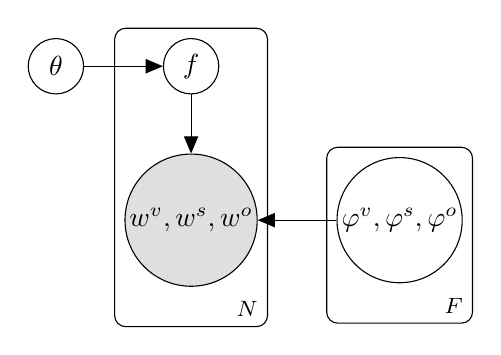
\begin{tikzpicture}
  % Nodes
  \node[obs] (datapoint) {$w^v,w^s,w^o$} ; %
  \node[latent, above=0.75cm of datapoint] (F) {$f$} ; %
  \node[latent, left=of F] (theta) {$\theta$}; %
  \node[latent, right=of datapoint] (phi) {$\varphi^v,\varphi^s,\varphi^o$}; %
  \edge {theta} {F} ; %
  \edge {F} {datapoint}
  \edge {phi} {datapoint} ; %
  \plate {tuples} {(F) (datapoint) } {$N$}; %
  \plate {} {(phi)} {$F$} ; %
\end{tikzpicture}


    \caption{Model 0}
    \label{gen0}

  \end{subfigure}
  \hfill
  \begin{subfigure}[b]{0.45\textwidth}

    \begin{snugshade}
    \scriptsize
    For each frame $f=1..F$:\\
    \hspace*{15pt} For each argument $a\in\{v,s,o\}$:\\
    \hspace*{30pt} Draw a distribution $\phi_f^a\sim Dirichlet(\beta)$\\
    For each document $d=1..D$:\\
    \hspace*{15pt} Draw a distrbution $\theta_d \sim Dirichlet(\alpha)$\\
    \hspace*{30pt} For each $i = 1..N^d$:\\
    \hspace*{30pt} Draw a frame $f \sim \theta^d$.\\
    \hspace*{30pt} Draw a verb $v \sim \phi_f^v$\\
    \hspace*{30pt} Draw a subject $s \sim \phi_f^s$\\
    \hspace*{30pt} Draw an object $o \sim \phi_f^o$
    \end{snugshade}

    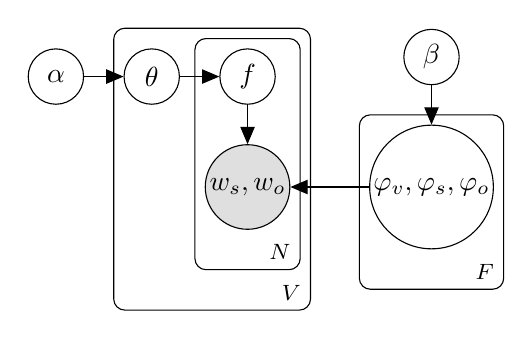
\begin{tikzpicture}[]
    \node[obs]                   (w)     {$w_s,w_o$}; %
    \node[latent, above=0.5cm of w]     (f)     {$f$};
    \node[latent, left=0.5cm of f]     (theta) {$\theta$};
    \node[latent, left=0.5cm of theta] (alpha) {$\alpha$};
    \node[latent, right=of w]    (phi)   {$\varphi_v,\varphi_s,\varphi_o$};
    \node[latent, above=0.5cm of phi] (beta) {$\beta$};
    \edge {alpha} {theta};
    \edge {theta} {f};
    \edge {f} {w};
    \edge {phi} {w};
    \edge {beta} {phi};
    \plate {frames} {(phi)} {$F$};
    \plate {datapoints} {(f) (w)} {$N$};
    \plate {verbs} {(f) (w) (datapoints) (theta)} {$V$};
\end{tikzpicture}


    \caption{Model 1}
    \label{gen1}

  \end{subfigure}

  \caption{Generative Stories}

\end{figure}



\subsection{Model 0}

The approach models each VSO independenly, without considering any further context.
Word distributions are completely independent between arguments and accross frames.
Tuples are clustered according to which frame's three distributions best fit the 
three arguments.

Model 0 is based on one originally proposed in \citet{rooth1999}, which 
considers noun-verb pairs. Following \citet{oconnor2013}, we expand the model
to use the limited syntax of VSOs.

The generative story (figure \ref{gen0}) gives us the following joint probability:
\begin{align*}
P(\mathbf{f},\mathbf{w}|\phi,\theta) 
  =& P(\mathbf{f}|\theta)P(\mathbf{w}|\phi)\\
  =& \prod_{i=1}^{N}\big[\theta(f_i) \prod_a^{\{v,s,o\}}\phi_{f_i}^a(w_i^a)\big]
\end{align*}

Therefore, the incomplete log-likelihood (i.e., where the sequence of frames
is hidden) that we want to maximize is as follows:
\[
L(\theta,\phi) = \sum_{i=1}^N\big[\log \sum_{f_i=1}^F\theta(f_i)\prod_{a}^{\{v,s,o\}}\phi_{f_i}^a(w^a_i)\big]
\]

Expectation maximization can be used to maximize this likelihood.
First we use the current estimates for $\theta$ and $\phi$ to infer a 
distribution over possible choices of frame. This is the E-step. 

\begin{align}
\mu_i(f) =& P(f_i=f, w_i|\phi,\theta)\nonumber\\
=& \frac{\theta(f)\prod_a^{\{v,s,o\}}\phi_f^a(w^a_i)}
                {\sum_{f'=1}^F\theta(f)\prod_a^{\{v,s,o\}}\phi_f^a(w^a_i)}\label{E}
\end{align}

Then in the M-step, we find $\theta$ and $\phi$ that maximize the expectation of
the complete likelihood. In particular, we want to maximize

\begin{align*}
E_\mu\big[\sum_{i=1}^N\log P(w_i,f_i|\theta,\phi)
=& \sum_{i=1}^N\sum_{f=1}^F\mu_i(f)\log\Big[\theta(f)\prod_a^{\{v,s,o\}}\phi_f^a(w_i^a)\Big]\\
=& \sum_{i=1}^N\sum_{f=1}^F\mu_i(f)\log\theta(f)
+ \sum_a^{\{v,s,o\}} \sum_{i=1}^N\sum_{f=1}^F\mu_i(f)\log \phi_f^a(w_i^a)
\end{align*}

Thus the problem is reduced to maximizing each of the terms in the sum above. Fortunately
these have closed for solutions using Lagrangian multipliers.


\begin{align}
\argmax_{\theta(f)}\sum_{i=1}^N\sum_{f=1}^F\mu_i(f)\log\theta(f)
= \frac{\sum_{i=1}^N\mu_i(f)}{\sum_{f'}^F\sum_{i=1}^N\mu_i(f)}
\end{align}

and

\begin{align}
\argmax_{\phi^a(w)}\sum_{i=1}^N\sum_{f=1}^F\mu_i(f)\log \phi_f^a(w_i,a)
= \frac{\sum_{i=1}^N \mu_i(f)\,c(w^a)}{\sum_{w'=1}^{V^a}\sum_{i=1}^N \mu_i(f)\,c(w',a)}
\end{align}

Where $c(w,a)$ indicates the number of times word $w$ is observed as argument $a$.

\subsection{Model 1}

It is in the nature of documents that they have some degree of internal semantic
coherence. Put more plainly, a document is usually \emph{about} something. We
know from topic modeling that LDA with Gibbs sampling can be very successful at
classifying documents according to some semantic features \citep{griffiths2004}.
Model 1 leverages this fact by making the assmumption that a given document is 
likely to have a sparse distribution of frames. As in LDA, the document-level
sparsity is enforced by a dirichlet prior on frame distributions (see figure
\ref{gen1} for details). This assumption breaks the independence between tuples 
that is maintained by Model 0 is dropped in Model 1.

The independence assumptions in the generative story for model 1 give us the 
following joint distribution:

\begin{align*}
P(\mathbf{w},\mathbf{f}|\theta,\phi,\alpha,\beta)
&=P(\mathbf{w}|\mathbf{f},\phi)\,P(\mathbf{f}|\theta)\,P(\theta|\alpha)\,P(\phi|\beta)
\end{align*}

We can find the marginal distribution of the latent and observed variables by
integrating over the priors:

\begin{align*}
 P(\mathbf{w},\mathbf{f}|\alpha,\beta)
&=\int_\phi\int_\theta P(\mathbf{w},\mathbf{f}|\theta,\phi,\alpha,\beta)\\
&=     \int_\phi P(\mathbf{w}|\mathbf{f},\phi )\,P(\phi|\beta)
\times \int_\theta P(\mathbf{f}|\theta)\,P(\theta|\alpha)\\
\intertext{These integrals are both dirichlet multinomials:}
&=\frac{DCM_i^{frames}(f_{ij}=f, \mathbf{f}_{-ij})}{DCM_i^{frames}(\mathbf{f}_{-ij})}\times
\prod_a^{\{v,s,o\}}\frac{DCM_i^{vocab^a}(f_{ij}=f, \mathbf{f}_{-ij})}{DCM_i^{vocab^a}(\mathbf{f}_{-ij})}
\end{align*}

We prefer not to consider the subject and object vocabularies independently 
(i.e., $V^s = V^o$). This is more in line with the theory of semantic frames 
since in principle, a noun playing a particlar semantic role may appear in either 
syntactic position.

Dropping terms not dependent on counts, we can calculate the proportional
probability required for Gibbs sampling as follows:

\begin{align}
P(f_{ij} = f|\mathbf{f}_{-ij},\mathbf{w}, \alpha,\beta)
&=\frac{\alpha + \tilde c(d_i,f)}{F\,\alpha + \tilde c(d_i)}
\times \prod_a^{\{v,s,o\}}\frac{\beta+\tilde c(f,w_{ij}^a)}{V^a\beta+\tilde c(f)}
\end{align}

Where $\tilde c (d_i, f)$ is the number of VSO's in document $d_i$ assigned to frame $f$;
$\tilde c(d_i)$ is the number of VSO's in document $i$;
$\tilde c(f,w_{ij}^a)$ is the number of VSOs containing $w_{ij}^a$ as argument $a$ that are
assigned to frame $f$; and
$\tilde c(f)$ is the number of VSOs assigned to frame $f$.
Note that $\tilde c$ indicates a count that does not consider the contribution of 
$w_{i,j}$.

The data used in this probject (see section \ref{data}) doesn't contain any document-level
information. As a result, we adapt model 1 by grouping VSOs with the same verb into ``documents''.
This move leverages the dirichlet prior $\alpha$ to enforce sparcity of frames 
accross verbs, but of course cannot capture the information given by the kind of
document-level semantic sparsity seen in LDA.\footnote{When we use verbs as
documents (i.e, $D = V^v$), since $w_{ij}^v$ is the same for all verbs in document $d_i$ 
(and $d_i$ is the only document with that verb), it follows that the number of VSO's in document 
$d_i$ belonging to frame $f$ is the same as the number of VSO's with $w_{ij}^v$ as their verb assigned to 
frame $f$; that is, $\tilde c(d_i, f) = \tilde c(f, w_{ij}^v)$.}

\section{Dataset - Verbargs}
\label{data}

A syntactic-ngram is a $k$-word rooted subtree of some sentence.
Google syntactic-ngrams is a corpus of ngrams extracted from 3.5 million English language 
books and labled with Penn Treebank part-of-speech tags Stanford-basic dependency 
lables \citep{ngrams2013}.
Each ngram also includes frequency counts by year.

This project uses the verbargs subeset (130M items) of Google syntactic-ngrams.
An ngram in the verbargs dataset consist of a verb and all of its 
immediate arguments.
We considered only the VSO's in this dataset, that is; we pruned verbargs to
those ngrams containing a subject (nsubj) and object (dobj) whose immediate parent
is the ngram's root verb (1.6M items, 96M by count). 
We further trimmed the data to consider only the \%25 most common verbs 
(800K items, 78M by count).



\section{Experiments}
The number of frames in both models must be determined before induction. When choosing for a low number of frames the clusters will be big and thus the meaning of a cluster vague. But a high number of frames has, next to high computational costs also a danger of overfitting the data. When unrelated verbs occur with the same arguments often they will be clustered and maybe will even make up one cluster, while with a lower number of frames other verbs would be included, diinishing one of the unrelated verbs as noise.

The alphas and betas are known \citep{oconnor2013} to be hard to determine, and therefore need experiments to be set to optimal values for a specific problem. We used, expensive but easy to implement, grid search to determine all parameters to test with. With grid-search a model is build with certain parameters, this model is then evaluated on a cross validation set. When all possible models are evaluated the highest scoring model is tested on. 

\section{Results}
\label{results}
\subsection{Frame Coherency}
rame coherency: for a datapoint $(v,s,o)$ and a tuple $(v^r,s,o)$ where $v^r$ is a random choses verb: $P(v\mid s,o) \geq P(v^r\mid s,o)$  
\subsection{Frame Correctness}
% I (Eli) can expond here on the relation/contrast/etc.
%   between what we're doing and Framenet;
%   I think O'Connor brings up some technical and/or methodological points
%   about ways we can vs. can't use the FN data for evaluating
%   induction and such, I'll look it over again.

Frame correctness: for the top 25 most probable verbs per frame $TV$ and framenet classes of verbs $FN$: \[\frac{2|TV\cap FN|}{|TV|+|FN|}\]

\subsection{Model 0}
\subsection{Model 1}


\section{Discussion}


\section{Future Work}
One big weakness of this project over the results of \citet{oconnor2013} is that 
we could not used document-level context to infer semantic information.
A possible direction of future reseach is to create models that take better 
advantage of the syntax-level context provided by syntactic ngrams. 
One easy way to do this would be to modify model 1 so that the argument 
vocabulary ranges over subject/object pairs instead of individual nouns.
or object.
More advanced models might take better advantage of the various kinds of arguments
in the verbargs dataset and their relation to one another.
For example, you could be gleen some semantic information about the relationship between
verbs and prepositional objects by looking at the preposition that mediates them: 
That you ''swim \emph{in} a lake'' versus ``ice skate \emph{on} a lake'' 
indicates that the relationship between swimming and lakes is different from the one between
ice skating and lakes.

\section{Conclusion}


\bibliography{refs.bib}

\end{document}
